\documentclass[conference]{IEEEtran}
\usepackage{cite}
\usepackage{amsmath,amssymb,amsfonts}
\usepackage{algorithmic}
\usepackage{graphicx, subfig}
\usepackage{textcomp}
\usepackage{xcolor}
\usepackage{listings}
\usepackage{hyperref}
\usepackage{float}

\def\BibTeX{{\rm B\kern-.05em{\sc i\kern-.025em b}\kern-.08em T\kern-.1667em\lower.7ex\hbox{E}\kern-.125emX}}

\begin{document}

\title{Manual ADS-B Communication Protocol Implementation on the ADALM-PLUTO Using GNURadio}

\author{
    \IEEEauthorblockN{Alan Manuel Loreto Cornídez}
    \IEEEauthorblockA{\textit{College of Electrical and Computer Engineering} \\
    \textit{The University of Arizona}\\
    Tucson, Arizona \\
    aloretocornidez@arizona.edu}
\and
    \IEEEauthorblockN{Jeremy Sharp}
    \IEEEauthorblockA{\textit{College of Electrical and Computer Engineering} \\
    \textit{The University of Arizona}\\
    Tucson, Arizona \\
    jeremysharp@arizona.edu}
}

\maketitle

\begin{IEEEkeywords}
  Software Defined Radio, ADS-B, GNURadio
\end{IEEEkeywords}

\begin{abstract}
%% Write Abstract Here

 

\end{abstract}



\section{Introduction}
%% Right now this is the proposal.
The most common method for aircraft to report their system state involves the use of the Automatic Dependent Surveillance-Broadcast (ADS-B) transmission method.
An open transmission method used to broadcast an aircraft's position, enabling the ability to track the aircraft.
Throughout the Spring 2024 semester, we have worked with the ADA Pluto Software Defined Radio (SDR) to receive and transmit signals in multiple ranges of frequency bands.
We have implemented pre-made signal processing blocks in GNURadio signal flow graphs and then implemented them on the ADA Pluto for applications such as FM Radio and AM radio.
Our project would like to work on solving the "1090 MHz Riddle".
What is the 1090 MHz Riddle you may ask? For many Software Defined Radio (SDR) enthusiasts, being able to capture, decode, interpret, and transmit ADS-B signals involves an understanding of how signals are are manipulated in the RF spectrum, both for transmission and modulation.
In our particular case, we would like to implement the use of the 1090 MHz frequency band to communicate with public aircraft information.
We have found pre-made GNURadio block that implement ADS-B communication protocols, however, we would like to explore a custom implementation using only a GNURadio signal flow graph and the QT GUI elements.
After implementing a simple receiver and transmitter, we would like to expand the project scope to receive real ADS-B signals transmitted by aircraft.
If this project goal is met, we would like to decode and interpret the data by plotting received data on a map.

\section{ADS-B Introduction}
The ADS-B protocol is a used to transmit information about an aircraft while the aircraft is in flight. 
The ADS-B can be used to transfer information about the aircraft's location, direction, and air speed. 
This protocol is used by aircraft in many places around the world such as the United States, Canada, Europe, and Australia. 
The United States made it a requirement to fly with ADS-B equipped aircraft in January 2020. 

\section{ADS-B Frame Structure}
Let us break down the frame structure of an ADS-B packet so that we can decode the information contained within. 

An ADS-B packet contains 112 bits. The packet contains 5 main parts. 5 bits are used for the downlink format of the aircraft, 3 bits are used to relay transponder capability information. 24 bits are used to transmit the ICAO aircraft address. 56 bits are used to transmit an extended squitter message. 5 bits are used to for a type code. Finally, the last 24 bits are used as an error check for the integrity of the packet using a cyclic redundancy check. As you can see in \autoref{fig:ads-b-bits}, provided by \cite{sun1090mhz}, the total amount of bits that are used in a ADS-B packer is 112. In addition to the use of the 112 bits in the message, there is also a 16 bit preamble used for frame synchronization.

% This is the table from https://mode-s.org/decode/content/ads-b/1-basics.html where the writer talks about the ads-b packet structure.
\begin{figure}
\begin{center}
\begin{tabular}{ | c | c | c | c | }
  Bit & No. Bits & Abbreviation & Information \\ 
  1–5 & 5 & DF & Downlink Format \\
  6–8 & 3 & CA & Transponder capability \\
  9–32 & 24 & ICAO & ICAO aircraft address \\
  33–88 & 56 & ME & Message, squitter \\
  (33–37) & (5) & (TC) & (Type code) \\
  89–112 & 24 & PI & Parity/Interrogator ID
\end{tabular}
\end{center}
\caption{A breakdown of an ADS-B packet.}\label{fig:ads-b-bits}
\end{figure}

%% Implementation
\section{Implementation}

Transmissions for ADS-B signals are made in the 1090 MHz frequency band which is within the capabilities of the ADALM-PLUTO, as such, the Pluto was used in our implementation. 
We wanted to have the best chances of implementing a successful solution for for both receiving and transmitting data, we decided to design and make custom antennas for the project.
After making our custom antennas, we wanted to do some initial testing with an MVP to make sure that data transfer was successful on the Pluto, because of this, we attempted to make two minimum viable products (MVPs) using different approaches.
The first approach involved the use of an ADS-B example provided by Mathworks in Matlab.
The second MVP was the use of a GNURadio out of tree module that contains ADS-B framing, demodulation, and decoding blocks.
After these two attempts were made, we created custom signal flow graphs that checked for an ADS-B frame preamble at the correct frequencies.
More information about the implementations can be found below.
Results for the complete implementation can be found in the Results section of the report.

%% Custom Antenna Design
\subsection{Custom Antenna Design}

%% Matlab Implementation
\subsection{Matlab Implementation}
 Using \cite{matlabAir} we created a working output that was able to read some mock data for an ADS-B transmissions.
In addition to helping us verify the ability to work with ADS-B signals in MATLAB, we were able to see how data is interpreted using an approach in code. 
However, the example given in the code was not useful in out manual implementation due to a lack of however level detail on ADS-B packet interpretation.

%% Out of Tree Modules for GNURadio
\subsection{Out of Tree Modules for GNURadio}
Another approach that we decided to implement was the use of an out-out-tree (OOT) module \cite{oot-adsb} in GNURadio.
To our surprise, there was already a GNURadio module available to help interpret received signals using the given framing, demodulating, and decoding, blocks given in the `gr-adsb` package.
From the example given in the repository for the OOT module shown in \autoref{fig:gr-adsb-example}, we can see that there are ADS-B Framer and ADS-B Demodulator blocks provided by the `gr-ads-b` OOT module. 

\begin{figure}
  \begin{center}
    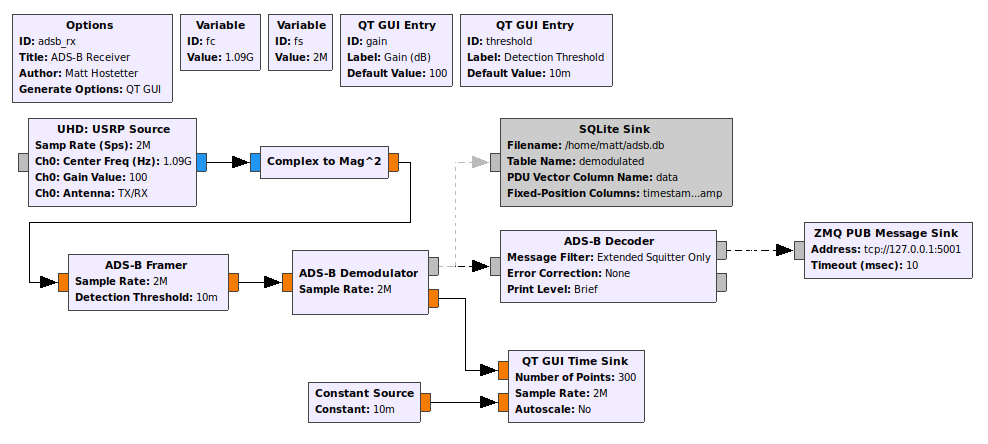
\includegraphics[width=0.5\textwidth]{./figures/adsb_rx.png}
  \end{center}
  \caption{A GNURadio signal flow graph that is given as an example in the git repo where the `gr-adsb` module is available.}\label{fig:gr-adsb-example}
\end{figure}

However, after multiple attempts trying to install the package on an arch-linux based system, python package management was not allowing us to work with the manually installed packages for the `gnuradio.adsb` python modules.
Regardless, we spent a bit of time looking at the source code of each of the modules to see how we would be able to implement similar function using individual blocks in GNURadio that are part of the Core package within GNURadio.

% So while the `gr-adsb` OOT module was not very helpful to us in in the sens





%% GNURadio Signal Flow Graphs
\subsection{GNURadio Signal Flow Graphs}


%% GNURadio Preamble
\subsection{GNURadio Preamble}

%% Procedure
\section{Procedure}

%% Results
\section{Results}

%% Problems with Frame Synchronization
\subsection{Problems with Frame Synchronization}

%% Conclusion
\section{Conclusion}





%% Generate the BibTeX bibliography.
\bibliographystyle{ieeetr}
\bibliography{refs}

\end{document}

